% ------------------------------------------
%  MASTER THESIS DISSERTATION
% ------------------------------------------
% Author:
%
% Advisors:
%
% ------------------------------------------
\documentclass[10pt,twoside,openright,a4paper]{report}
\usepackage[utf8]{inputenc}

% Set document margins to 1in in all sides
\usepackage[margin=2.5cm]{geometry}
% Line spacing package
\usepackage{graphicx, helvet, hyperref, setspace}
\usepackage{epstopdf}
\usepackage[portuguese,english]{babel}
\usepackage[acronym, toc, nonumberlist]{glossaries}
% Extra stuff file
% This file is included before begin{document} environment
% Use this to include extra packages and define your own commands
% This way, you can easily grab a most recent version
% of dissertation.tex file from the original repo

\newcommand{\chapquote}[3]{\begin{quotation} \textit{#1} \end{quotation} \begin{flushright} - #2, \textit{#3}\end{flushright} }

%%%%%%%%%%%%% GDL listings %%%%%%%%%%%%%%%%%%%

\usepackage{listings}
\usepackage{color}

\definecolor{keywordcolor}{rgb}{0,0.4,0.7}
\definecolor{numbercolor}{rgb}{0.8,0.3,0}
\definecolor{commentcolor}{rgb}{0.4,0.4,0.4} 	
\definecolor{mygray}{rgb}{0.5,0.5,0.5} 	% line counter color
\definecolor{mymauve}{rgb}{0.55,0.28,0.62}	% string color
\definecolor{codebackground}{rgb}{0.97,0.97,0.97} 

\lstset{ %
  backgroundcolor=\color{codebackground},   % choose the background color; you must add \usepackage{color} or \usepackage{xcolor}
  basicstyle=\ttfamily \footnotesize,        % the size of the fonts that are used for the code
  breakatwhitespace=false,         % sets if automatic breaks should only happen at whitespace
  breaklines=true,                 % sets automatic line breaking
  captionpos=b,                    % sets the caption-position to bottom
  commentstyle=\color{commentcolor},    % comment style
  deletekeywords={...},            % if you want to delete keywords from the given language
  escapeinside={\%*}{*)},          % if you want to add LaTeX within your code
  extendedchars=true,              % lets you use non-ASCII characters; for 8-bits encodings only, does not work with UTF-8
  keepspaces=true,                 % keeps spaces in text, useful for keeping indentation of code (possibly needs columns=flexible)
  keywordstyle=\color{keywordcolor},       % keyword style
  numbers=left,                    % where to put the line-numbers; possible values are (none, left, right)
  numbersep=5pt,                   % how far the line-numbers are from the code
  numberstyle=\tiny\color{mygray}, % the style that is used for the line-numbers
  rulecolor=\color{black},         % if not set, the frame-color may be changed on line-breaks within not-black text (e.g. comments (green here))
  showspaces=false,                % show spaces everywhere adding particular underscores; it overrides 'showstringspaces'
  showstringspaces=false,          % underline spaces within strings only
  showtabs=false,                  % show tabs within strings adding particular underscores
  stepnumber=1,                    % the step between two line-numbers. If it's 1, each line will be numbered
  stringstyle=\color{mymauve},     % string literal style
  tabsize=2                       % sets default tabsize to 2 spaces
}

\lstdefinelanguage{GDL}{%
  language = Prolog,
  keywordsprefix=?,
  %
  keywords = [2]{init, cell, next, does, role, control, mark, distinct, goal, terminal, legal},
  keywordstyle=[2]\color{mymauve},
  morecomment=[l]{;},
}

\newtoggle{InString}{}% Keep track of if we are within a string
\togglefalse{InString}% Assume not initally in string

\newcommand*{\ColorIfNotInString}[1]{\iftoggle{InString}{#1}{\color{numbercolor}#1}}%
\newcommand*{\ProcessQuote}[1]{#1\iftoggle{InString}{\global\togglefalse{InString}}{\global\toggletrue{InString}}}%
\lstset{literate=%
    {"}{{{\ProcessQuote{"}}}}1% Disable coloring within double quotes
    {'}{{{\ProcessQuote{'}}}}1% Disable coloring within single quote
    {0}{{{\ColorIfNotInString{0}}}}1
    {1}{{{\ColorIfNotInString{1}}}}1
    {2}{{{\ColorIfNotInString{2}}}}1
    {3}{{{\ColorIfNotInString{3}}}}1
    {4}{{{\ColorIfNotInString{4}}}}1
    {5}{{{\ColorIfNotInString{5}}}}1
    {6}{{{\ColorIfNotInString{6}}}}1
    {7}{{{\ColorIfNotInString{7}}}}1
    {8}{{{\ColorIfNotInString{8}}}}1
    {9}{{{\ColorIfNotInString{9}}}}1
}

%%%%%%%%%%%%% GDL listings %%%%%%%%%%%%%%%%%%%

% Built the glossary when the main file is built.
\makeglossaries
% Set main font to Arial
\renewcommand{\familydefault}{\sfdefault}
% Define keywords macro
\providecommand{\keywords}[1]{\textbf{Keywords:} #1}
% Define "palavras-chave" macro
\providecommand{\palavrasChave}[1]{\textbf{Palavras-Chave:} #1}
% Define the NewPage macro
\newcommand*\NewPage{\newpage\null\thispagestyle{empty}\clearpage}
% Abstract-en page numbering
\newcommand {\abstractEnglishPageNumber} {\thispagestyle{plain}\setcounter{page}{\abstractEnglishPage}}
% Abstract-pt page numbering
\newcommand {\abstractPortuguesePageNumber} {\thispagestyle{plain}\setcounter{page}{\abstractPortuguesePage}}
% Section numbering depth
\setcounter{secnumdepth}{3}
% Table of contents depth
\setcounter{tocdepth}{3}
% Set line spacing to 1.5cm
\onehalfspacing
% Page numbering
\pagestyle{plain}

% Glossary-File
% Glossary Definition

\newglossaryentry{MSc}{name={MSc}, description={Masters degree in the area of Science.}}

\newglossaryentry{Reasoner}{name={Reasoner}, description={The component of a GGP player that interprets GDL game rules}}

\newglossaryentry{Game Manager}{name={Game Manager}, description={The system that acts as a referee on a GGP match}}

% Acronym-File
% Acronym Definition

\newacronym{IST}{IST}{Instituto Superior T\'ecnico}

\newacronym{AI}{AI}{Artificial Intelligence}
\newacronym{GGP}{GGP}{General Game Playing}
\newacronym{MCTS}{MCTS}{Monte Carlo Tree Simulation}
\newacronym{UCT}{UCT}{Upper Confidence Bounds applied for Trees}
\newacronym{GDL}{GDL}{Game Description Language}
\newacronym{MDP}{MDP}{Markov Decision Problem}


% ------------------------------------------
% MASTER THESIS DISSERTATION
% ------------------------------------------

\begin{document}
\pagenumbering{gobble}% Remove page numbers (and reset to 1)
\clearpage
\thispagestyle{empty}
%!TEX root = ./dissertation.tex

% Dissertation basic information
\newcommand {\Title} {General Game Playing}
\newcommand {\Subtitle} {Adaptable, Multi-Game Playing Programs}
\newcommand {\StudentName} {Ricardo Filipe Amendoeira}
\newcommand {\DegreeName} {Electrical and Computer Engineering}
\newcommand {\Supervisors} {{\large Prof. Nuno Cavaco Gomes Horta}

							{\large Prof. João Paulo Carvalho}}

% Include or not include acknowledgments
\def \includeAcknowledgments{0}

% Include or not include glossary
\def \includeGlossary{0}

% Examination Committee
\newcommand {\Advisor} {{\large Prof./Dr. Lorem Ipsum}}
\newcommand {\CoAdvisor} {{\large Prof./Dr. Co Advisor}}

% After the thesis defense
\newcommand {\CommitteeMembers} {
{\large Prof./Dr. Lorem Ipsum}\\
{\large Prof./Dr. Lorem Ipsum}
}
\newcommand {\Chairperson} {{\large Prof./Dr. Lorem Ipsum}}

% Is final version (will include Committee Members information)
\def \IsFinalVersion{0}

% Date
\newcommand {\Month} {December}
\newcommand {\Year} {2015}

% Acknowledgments page number
\def \acknowledgmentsPage{1}

% Abstract-en page numbering
\def \abstractEnglishPage{3}

% Abstract-pt page number
\def \abstractPortuguesePage{5}

% You had a co-advisor:
\def \HasCoAdvisor{0}

% Logo Spacing Variables
\def \finalLogoSpacing{2.0cm}
\def \draftLogoSpacing{2.0cm}

% Advisors Spacing Variables
\def \finalAdvisorsSpacing{1.0cm}
\def \draftAdvisorsSpacing{10.0cm}

% Date Spacing Variable
\def \dateSpacing{5.0cm}

% You can define your own variables here


%!TEX root = ./dissertation.tex

% ---------------------------------------------------------
%   MASTER THESIS DISSERTATION COVER
% ---------------------------------------------------------
\begin{titlepage}
% ---------------------------------------------------------
%  INSTITUTION LOGO
% ---------------------------------------------------------

\includegraphics[width=5cm]{images/ist_logo}~\\
%
\if\IsFinalVersion 1
  \vspace*{\finalLogoSpacing}
\else
  \vspace*{\draftLogoSpacing}
\fi

\begin{center}
% ---------------------------------------------------------
%  MASTER THESIS DISSERTATION TITLE
% ---------------------------------------------------------
{\LARGE \textbf{\Title}}\\[1.0cm]
% ---------------------------------------------------------
%  MASTER THESIS DISSERTATION SUBTITLE
% ---------------------------------------------------------
{\Large \Subtitle}\\[1.0cm]
% ---------------------------------------------------------
%  AUTHOR NAME (FULL)
% ---------------------------------------------------------
{\Large \textbf{\StudentName}}\\[1.0cm]
% ---------------------------------------------------------
%  DISSERTATION DEGREE
% -----------------------------------------------------------------
{\large Thesis to obtain the Master of Science Degree in}\\[1.0cm]
% -----------------------------------------------------------------
%  COURSE NAME
% -----------------------------------------------------------------
{\LARGE \textbf{\DegreeName}}\\[1.0cm]

% -----------------------------------------------------------------
%  ADVISORS NAME
% ---------------------------------------------------------
\begin{minipage}[t]{.4\textwidth}
  \center
  \begin{flushright}
    {\large Supervisors:~~}
  \end{flushright}
\end{minipage}%
\begin{minipage}[t]{.6\textwidth}
  \center
  \begin{flushleft}
    {\Supervisors}
  \end{flushleft}
\end{minipage}\\
%
\if\IsFinalVersion 1
  \vspace*{\finalAdvisorsSpacing}
\else
  \vspace*{\draftAdvisorsSpacing}
\fi
% ---------------------------------------------------------
%  JURI NAMES:
%  - PRESIDENT
%  - ADVISOR
%  - VOGALS
% ---------------------------------------------------------
%
\if\IsFinalVersion 1
%
\begin{minipage}[t]{1\textwidth}
  \center
  {\Large \textbf{Examination Committee}}\\[.25cm]
  {\large Chairperson: \Chairperson}\\
  {\large Supervisor: \Advisor}\\
  {\large Member of the Committee: \CommitteeMembers}
\end{minipage}\\[1.0cm]
%
\fi
%

\if\IsFinalVersion 1
 \vspace*{\dateSpacing}
\fi

% ---------------------------------------------------------
%  DATE (MONTH AND YEAR)
% ---------------------------------------------------------
{\Large \textbf{\Month\:\Year}}\\
\end{center}
\end{titlepage}

\NewPage

\pagenumbering{roman}

\if\includeAcknowledgments 1
%!TEX root = ../dissertation.tex

% Acknowledgments: This one is optional
\chapter*{Acknowledgments}
% Thanks to everyone and bla bla bla

\NewPage
\fi

%!TEX root = ../dissertation.tex

\begin{otherlanguage}{english}
\begin{abstract}
% Set the page style to show the page number
\thispagestyle{plain}
\abstractEnglishPageNumber
Artificial Intelligence research has lead to many systems that perform incredibly well for the specific task they were designed for, but are useless for anything else.
For example, while Deep Blue could defeat Garry Kasparov, the world's chess champion, it was utterly incapable of playing checkers or even tic-tac-toe. Also, with these systems, all the interesting analysis of the game is done ahead of time and is done by the developers, not the system.
General Game Playing (GGP) aims to create computer systems capable of playing any game without human assistance, being given only the game rules. Such systems must be highly adaptable and should be capable of high-level tasks such as reasoning, learning or deduction, among others.
Player performance is dictated by how well it handles the following three tasks:
Interpreting the game rules (efficiently representing this knowledge), analyzing the game rules (recognizing patterns and other features) and deriving a strategy for the given game (quickly searching through the possible actions). 
%These tasks depend on three characteristics: How efficiently does the system represent it's knowledge, how deep it's analysis of the rules goes and how fast it can search through the possible moves for the game.

In this work an overview of GGP is given and the state of the art solutions are presented.


% Keywords
\begin{flushleft}

\keywords{}
General Game Playing,
Multi-Game Playing,
Artificial Intelligence,


\end{flushleft}

\end{abstract}
\end{otherlanguage}

\NewPage
%!TEX root = ../dissertation.tex

\begin{otherlanguage}{portuguese}
\begin{abstract}
\abstractPortuguesePageNumber
A investigação em Inteligência Artificial tem criado muitos sistemas com desempenho excepcional para as funções específicas para que foram desenhados, mas que são inúteis para qualquer outra função. Por exemplo, embora o Deep Blue tenha conseguido derrotar Garry Kasparov, o campeão mundial de xadrez, era completamente incapaz de jogar damas ou mesmo o tic-tac-toe. Para além disso, com estes sistemas, toda a análise interessante é feita previamente e é feita por quem desenvolve o sistema.
General Game Playing (GGP) tem como objectivo a criação de sistemas capazes de jogar qualquer jogo sem assistência humana, recebendo apenas as regras do jogo.
Sistemas deste tipo têm deser capazes de fazer tarefas de alto-nível como raciocinar, aprender e deduzir, entre outras. 
O desempenho de um jogador é ditado pela qualidade com que é capaz de executar as três seguintes tarefas: Interpretar as regras do jogo (representando de forma eficiente o conhecimento obtido), analizar as regras do jogo (reconhecendo padrões e outras características) e criando uma estratégia para esse jogo (fazendo uma pesquisa rápida pelas acções possíveis).

Neste trabalho é dada uma visão geral de GPP e o estado da arte da àrea é apresentado.


% Keywords
\begin{flushleft}

\palavrasChave{General Game Playing, Planeamento em Múltiplos Jogos, Inteligência Artificial}

\end{flushleft}

\end{abstract}
\end{otherlanguage}

\NewPage

% Table of contents
\tableofcontents
% A new page is necessary only if table of contents has an odd number of pages
%\NewPage

% List of tables
\addcontentsline{toc}{chapter}{\listtablename}
\listoftables
% A new page is necessary only if list of tables has an odd number of pages
\NewPage

% List of figures
\addcontentsline{toc}{chapter}{\listfigurename}
\listoffigures
% A new page is necessary only if list of figures has an odd number of pages
\NewPage

% List of acronyms
%\printglossary[type=\acronymtype]

\pagenumbering{arabic}% Arabic page numbers (and reset to 1)

%!TEX root = ../dissertation.tex

% Entry point for chapters
% In this file you define the order
% in which the chapters are included

% Chapters
% !TEX root = ../dissertation.tex

\chapter{Introduction}
\label{chapter:introduction}

\section{Motivation}

Game playing has always been a fundamental part of Artificial Intelligence (AI) research, as it can be used to test strategy in a straightforward way. Different games can be created to test specific features or properties that are of research interest, such as opponent modeling.

Throughout the history of AI research there was always a big focus on the ability of playing specific games, like chess, well. This focus led to systems like Deep Blue (the computer system that defeated Garry Kasparov at chess in the 90’s) that, while very advanced on the games they are designed for, delegate all the interesting analysis to the system designers. These systems are also completely useless for all games other than the one they were designed for (even if the difference is very small).

This over-specialization limits the usefulness of these systems. It is then of our interest to also be able to design more general systems, which could be closer to one of the most powerful features of human intelligence, adaptability:

\chapquote{``A human being should be able to (...) design a building, write a sonnet, balance accounts, build a wall, set a bone, comfort the dying, take orders, give orders, cooperate, act alone, solve equations, analyze a problem, pitch manure, program a computer, fight efficiently, die gallantly. \\ Specialization is for insects.''}{Robert A. Heinlein}{Time Enough for Love}

\gls{GGP} aims to develop general game playing systems, systems that can play any game when given the rules, acting as a stepping stone for General Intelligence research. Artificial General Intelligence has been a topic for science-fiction stories and, if possible, can be the biggest revolution in human history, allowing for an unprecedented ability of problem-solving.

\section{Multi-game playing}

Multi-game playing is the concept of developing programs that can play not just one, but many different games. This is not to be mistaken with combining many programs into one, multi-game players should be able to adapt to games unknown to them as well. Doing this requires many traits shared by \textit{Artificial Intelligence} research, such as deduction, reasoning, problem solving, intelligent search, knowledge representation, planning and learning.

General Game Playing was proposed in 2005 by Standford University as a platform for multi-game playing research, along with a language for describing games, the \gls{GDL}. An online course was created by Standford University and there are several new GGP projects every year, as well as various competitions, the biggest one being the annual GGP competition, held at the AAAI conference.

More recently another platform also appeared, General Video-Game Playing (GGVP), which focuses on video games.

\subsection{Early attempts at multi-game playing}

Possibly the earliest work on the subject was done in 1969 in \cite{Pitrat1969}. There were other notable works in the 90's, like SAL, Hoyle, Morph, METAGAMER (all sumarized in \cite{Mandziuk2013}) and Zillions of Games. Hoyle is described in more detail below.

\subsubsection{Hoyle}
A system developed in the 90’s, using a training scheme called lesson and practice, where lessons are games played against an expert and practice is self-playing. Predates GDP and was developed for 2-player games. The system used a set of game independent Advisers, each specialized in a game aspect such as position. These Advisers could recommend moves that could then be chosen by higher tier advisers. There were 3-tiers, depending on specialization:

\begin{enumerate}

\item [1st.] These Advisers specialized in immediate consequences: they performed very shallow searches to avoid things like instant loss moves. These decisions were final.

\item [2nd.] Advisers in this tier chose moves according to certain goals. These decisions were also final.

\item [3rd.] Advisers in the last tier differed from the first tiers in an important way: The decision of each Adviser wasn’t final, the final decision was decided by a process similar to taking a vote between the Advisers in this 3rd tier. Advisers votes were weighted in accordance to the lesson and practice results: Advisers that were more often correct during the training stage received bigger weights.

\end{enumerate}
This process of weighting the Advisers was crucial to the performance of the system and could even be worse than a random player if done incorrectly. If none of the 3rd tier advisers were even remotely related to the game being played the results would also be disappointing. Having a varied pool of Advisers was for this reason vital but they were never, by definition, general enough to be useful for any game. Hoyle was tested in 18 two-player board games, its potential in complex games was never verified.


\section{Objectives}

\paragraph{Main Objectives:}
\begin{itemize}
\item Research and compare current techniques and solutions for GGP players
\item Improve or develop new techniques for game playing
\item Use the improvements to make a new GGP player
\item Benchmark the player against other existing GGP players
\end{itemize}

\paragraph{Secondary Objectives:}
\begin{itemize}
\item Publish the results
\item Take the online course on GGP
\item Enter the annual GGP competition
\item Enter other relevant competitions
\end{itemize}


% A demonstration of how to use acronyms and glossary:

% A \gls{MSc} entry.

% Second use: \gls{IST}.

% Plurals: \glspl{MSc}.

% A citation example \cite{nobody}

%TEX root = ../dissertation.tex

\chapter{Background}
\label{chapter:background}

\section{The basics of General Game Playing}

General Game Playing is a project of the Stanford Logic Group of Stanford University, California, which aims to create a platform for \gls{GGP}.
Since 2005, there have been annual \gls{GGP} competitions at the AAAI Conference.

A \gls{GGP} match consists of 3 major components:
\begin{itemize}
\item Game Description: The game rules, in \gls{GDL}.

\item Game Manager: This system acts as a referee and manages communication with the players and other systems like graphics for the spectators. \textit{State Data} is usually part of the Game Manager.

\item Players: Players are the most interesting component of a \gls{GGP} game, they need.

\end{itemize}

\begin{figure}[h]
	\centering
    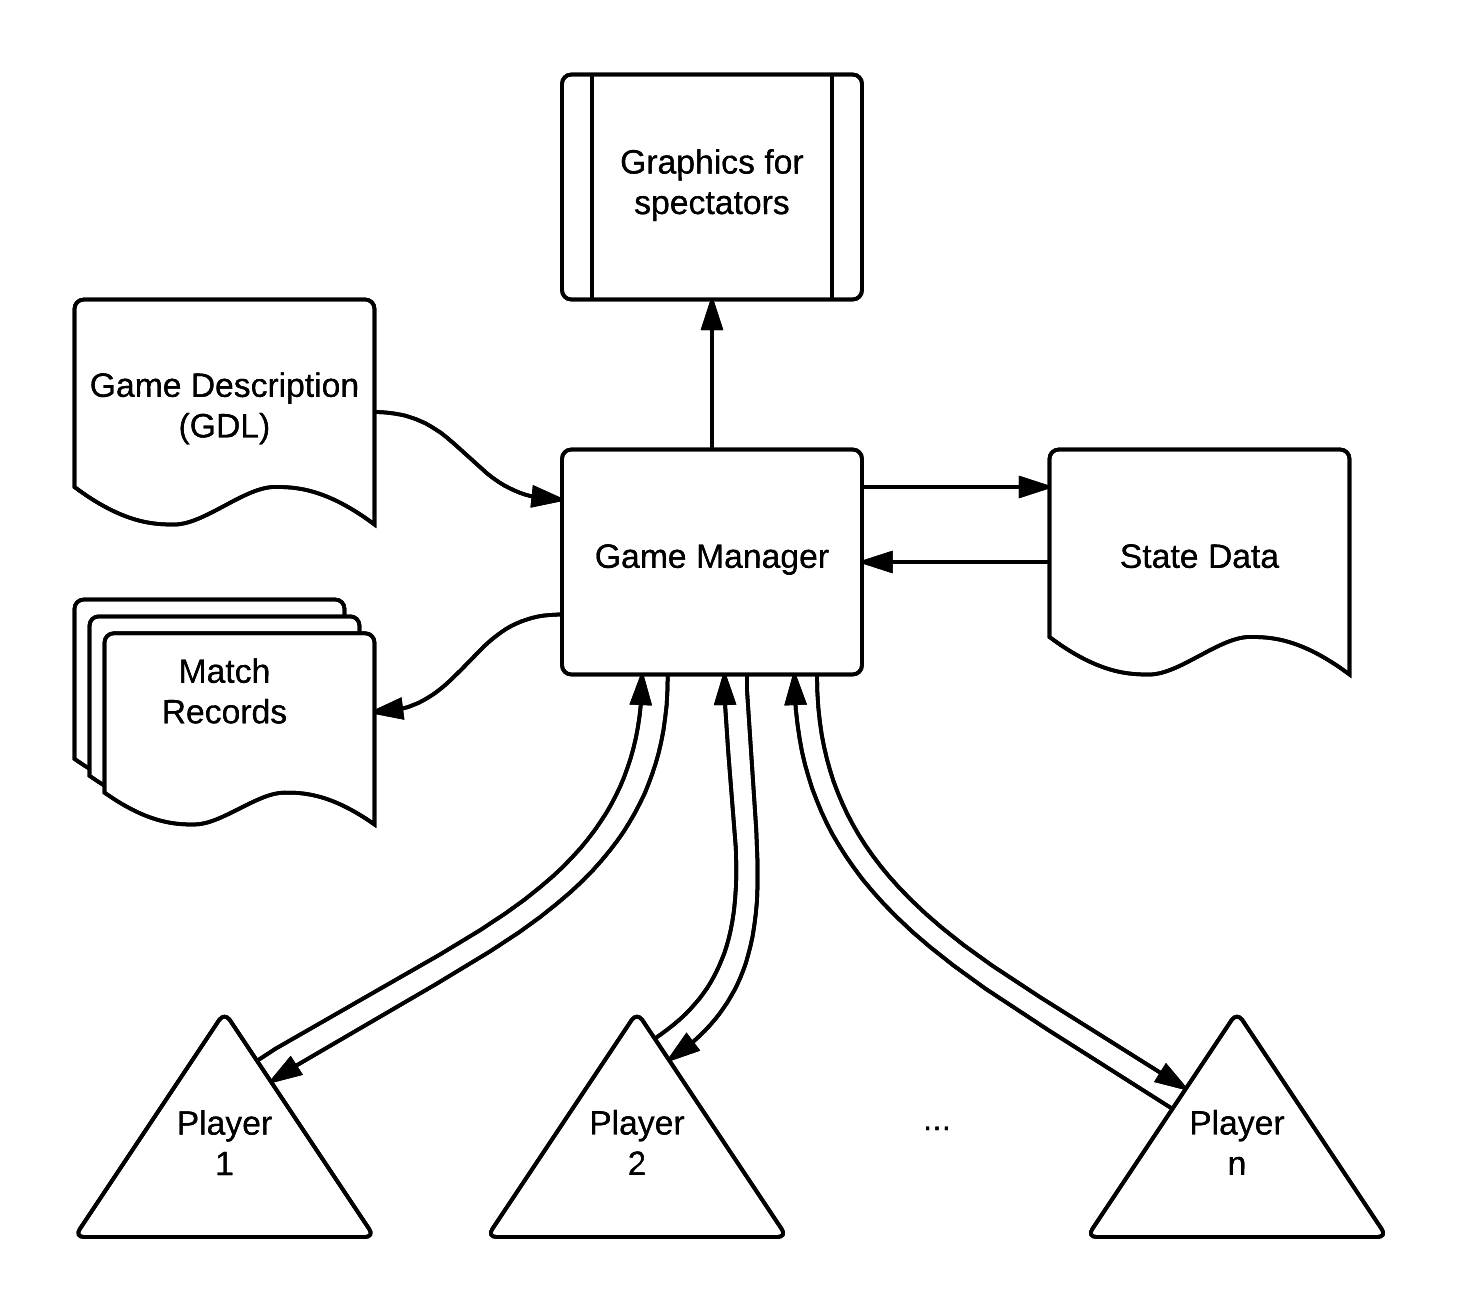
\includegraphics[scale=0.8]{images/GGPgamesetup.png}
    \caption{Match Components}
    \label{fig:match components}
\end{figure}

At the beginning of a match, the Game Manager sends all Players a match identifier, the game description, the role of each player and the time limits (for preparation (\textit{startclock}) and for each round (\textit{playclock})).

The match commences, after all players respond, with the Game Manager requesting a move from all players. Each round ends when all players send their moves or the time limit runs out (a random legal move is chosen for players that don't respond in time), after which the Game Manager will send each player another request along with all moves taken in the previous round.


\subsection{Game Description Language}
The \gls{GDL} is the standard way of describing games in the \gls{GGP} community.
\gls{GGP} players interpret the language using something called a \textit{Reasoner}. Choosing a good way of interpreting the game rules is one of the keys to performance and so many players develop their own custom \textit{reasoners}.

It can describe any finite deterministic move-based strategy game with an arbitrary number of players (most board games). GDL-II is an extension that has been made to allow for probabilistic games and incomplete information, like most card games.

Both GDL and GDL-II are variants of Datalog (query and rule language similar to prolog) and use first order logic.
Since GDL is a very conceptual description of the rules their interpretation is very computationally expensive. Choosing a good way of doing this interpretation (components that do this are called reasoners) is therefore very important to player performance, even in the recent years.

An example of tic tac toe described in GDL with some syntax explanation can be seen in \ref{appendix:gdl_example}

\subsection{Game Manager}
The purpose of the Game Manager is to be a single source of truth about what's happening in a match, and verify all moves taken by players. It must be able to interpret \gls{GDL}, to verify these moves

Players communicate their moves to the Game Manager (via HTTP), who checks the validity of the moves. A random legal move is chosen if a player chooses an illegal move or doesn't respond in time.

It should also provide a way of archiving the match history (all game states and moves taken) and other useful features like an interface for spectating.

\subsection{Game Player}
Game Players are systems that can interpret a \gls{GDL} game description, communicate with the Game Manager and devise strategies, to maximize their result in a certain game.

Game Players are, of course, the most interesting part of any \gls{GGP} match. Their aim is to be as general as possible while also having reasonably good performance in any game, which is a surprisingly difficult feat. Suffice it to say, sophisticated AI techniques like heuristics are very hard to successfully apply in a general, domain independent, way. So far, 
The most relevant techniques are discussed in chapter \ref{chapter:state_of_the_art}.

\section{Player components}

\subsection{Markov Decision Problem}

\section{Techniques}
\subsection{Monte Carlo Tree Search}
Introduced to the GGP competition by CADIA player in 2007, It’s currently the most used and successful method in GGP. Starting from the current state, the algorithm traverses the tree until the move timer ends, doing as many iterations as possible.

Each iteration has four steps: selection, expansion, simulation and back propagation:

\begin{enumerate}

\item Selection: Some technique is used to select which already traversed node to start from for a search. The most common technique is Upper Confidence Bounds applied for Trees (UCT), which includes a constant that can be tweaked to favor more or less exploration of non visited branches. The UCT algorithm is described in \ref{UCT}:

\begin{center}
\begin{equation} \label{UCT}
a^{*} = arg \max_{a\in A(s)} \left \{ Q(s,a) + C \sqrt{\frac{\ln|N(s)|} {N(s,a)}} \right \}
\end{equation}
\end{center}

Where $a^{*}$ is the selected node, $a \in A(s)$ means an action that contained in the set of possible actions in the current state $s$, $Q(s,a)$ is an assessment of performing $a$ in state $s$, $C$ is the exploration ratio constant, $N(s)$ is the number of previous visits to state $s$ and $N(s,a)$ is the number of times $a$ has been sampled in state $s$.

\item Expansion: Adding a node with the first unvisited state yet to the tree, meaning a state that wasn’t already in the tree.

\item Simulation: Perform a random simulation until a terminal game state is reached.

\item Back-Propagation: The scores obtained by all players at the end of the simulation are back-propagated to all nodes traveled in the selection and expansion stages.

\end{enumerate}

The success of MCTS can be mostly attributed to it not requiring any game-specific knowledge, although this can become a problem if other techniques like heuristics become advanced enough at learning important features of games, as heuristic search can be much faster than simulation. MCTS also has the advantage of parallelizing well. The biggest problems for MCTS are games that can have infinite moves without ending and tree size.

There have been several suggested improvements to the basic MCTS, although most aren’t very thoroughly tested yet. One of the most interesting ones is Simulation Heuristics, proposed by MINI-Player, which aims to add some sort of learning to the standard MCTS algorithm. The heuristics proposed are very light-weight and are the following:

\begin{itemize}

\item Random: The standard MCTS

\item History Heuristic: Tries to identify globally good actions (generally good regardless of state)

\item Mobility: Favors actions that lead to states with more move options relatively to other players.

\item Approximate Goal Evaluation: Tries to calculate the degree of satisfaction of a GDL goal rule. 

\item Exploration: Measures the difference between states as a way to do a diverse exploration. 

\item Statistical Symbol Counting: Before the start clock simulations are done to calculate the correlation between game score and certain game symbols (moves, pieces, board locations, etc). Symbols that do not change much are then ignored to allow more computation to be made on the more relevant ones.

\end{itemize}

\subsection{AI-Based Techniques}
Although currently not competitive with MCTS, there are several different approaches more similar to classical AI. Some of these are attempts at multi-game playing that predate GGP. These are techniques that try to learn or identify features of the game. One of the biggest drawbacks of this type of technique is that no general heuristic exists, meaning heuristics have to be discovered at run time, which is a very complex problem.


\chapter{State of the Art}
\label{chapter:state_of_the_art}

\section{Competition as a benchmark}
The General Game Playing annual competition has been, since its creation in 2005 in Stanford University, the way to know which methods are the state of the art. 
While in the early years of the competition there was a bigger focus on intelligent heuristics, Monte Carlo Tree Search (MCTS) has dominated the competition ever since, since it’s domain independent (general), inherently parallel and has shown better performance in most of the tested games. One of the most important features of MCTS is that the process of building the tree can be paused when necessary (for example when a turn ends) and continued at a later time. This allows a player to continue the simulations throughout the whole game, without restarting after each turn.
The variant of MCTS commonly used in GGP is called Upper Confidence Bounds Applied for Trees (UCT), which provides a simple method to balance tree exploration (search new branches) and exploitation (search deeper in the known branches). 

There are other, smaller, \gls{GGP} competitions that usually have the same results in terms of what techniques tend to perform best.


\section{State of the art players}

(Improve this section after doing more research on the solutions)
(reverse table axis, to be able to fit more information)

Qualified Players for the 2015 Main Competition

\begin{tabular}{| c | p{1cm} | p{3cm} | p{3cm} | p{3cm} | c | p{2.5cm} |}
\hline
  Name & Result & Reasoner & Planner & Additional \par Heuristics & Implementation & Creators \\
\hline
  Sancho & a & Prop. Network & MCTS with UCT & Yes, \par determined during game setup time & a & Steve Draper \par Andrew Rose \\
\hline
  Galvanise & a & Prop. Network & MCTS with UCT & a & a \\
\hline
  General & a & a & a & a & a\\
  \hline
  QFWFQ & a & a & a & a & a \\
  \hline
  Alloy & a & a & a & a & a \\
\hline
  TurboTurtle & a & a & a & a & a \\
  \hline
  QuorumPlayer & a & a & a & a & a \\
    \hline
  LeJoueur & a & a & a & a & a \\
  \hline
  SteadyEddie & a & a & a & a & a \\
  
\hline
\end{tabular}



\subsection{FluxPlayer}
The winner of the second GGP competition, in 2006, this player used fuzzy logic to determine how close to terminal a certain state is.

Fuzzy logic is a form of logic that allows multiple different values beyond True or False, and also allows overlap between these values. For example: water can be considered cold, warm or hot, but also warm and hot at the same time, since for some temperatures it is not clear which one is the correct one. Fuzzy logic also allows each of these states to have varying degrees of certainty: the water can be 80\% warm and 10\% cold, allowing conditions like if water is very warm: add some cold water, where the very keyword is also part of the fuzzy logic implementation.

The system also used a novel heuristic search that could be computed from the specifications of the game.

\subsection{Cadia Player}
Winner in 2007, started the reign of MCTS players in GGP.

\subsection{Sancho}
Champion in 2014, info here, need to research it: \url{http://sanchoggp.blogspot.pt/2014/05/what-is-sancho.html}

MCTS player with a few notable changes:
- propositional-network-based state machine (based on Petri Networks)
- general graph instead of MCTS tree
- some heuristics determined at game setup time

\subsection{Galvanize}
This years champion, MCTS based, research it:
\url{https://bitbucket.org/rxe/galvanise_v2}

\subsection{comparison}
research the top players from here:
\url{http://www.ggp.org/view/tiltyard/players/}
and here:
\url{https://docs.google.com/spreadsheets/d/12SWEXYAmCCGCm5jI-e0t1HGlMFXXeKSgyuU1boTioJ4/edit#gid=0&vpid=A1}
and make a comparison table.
If possible, run some of them and do my own comparisons.





\chapter{Preliminary results and planning}
\label{chapter:preliminary_results}

\section{Preliminary results}

To get a better understanding of the GGP platform, a few tests were run, using the application \textit{Kiosk} as a game manager (provided by ggp.org) and a few different game players:

\begin{itemize}

\item Sancho

\item Example MCTS+UCT player with Propositional Networks (tried different exploration bias values)

\item Example MCTS+UCT player with a Prolog reasoner

\item Example Mini-Max player with Alpha-Beta prunning and a Prolog reasoner

\item Example Mini-Max player without Alpha-Beta prunning and a Prolog reasoner

\item Example random legal player

\item A few other small variations of the example players, like enabling state caching on all of them.

\end{itemize}

Games on the \textit{Kiosk} application have graphical user interfaces and even allow a user to play directly against a player.
A few of the tested players were created by mixing and matching different software components already provided by ggp.org.

Overall, it was quite useful to get some practical knowledge on the field but performance comparisons proved to be quite laborious (many different games have to be tested for the results to have meaning) and so were avoided since better options already exist, namely the Tiltyard game server. Even so, in the small sample of games tested, Sancho was noticeably much better than the example players and myself, remaining unbeaten in games where it didn't run out of RAM (it was running on a machine with 6GB of RAM versus the 32GB it runs on for competitions).

\section{Planning}

\subsection{Work proposal}
From the research made in chapter \ref{chapter:state_of_the_art} it seems the most significant ways to advance \gls{GGP} research is to develop improvements to Propositional Network techniques and/or run-time creation of heuristics based on game rule analysis and so these will be the focus of the dissertation.

\subsection{Objectives and timeline}

\begin{table}[h]
\caption{Planned dates for the objectives}
\label{table:Planning}
\small
%\begin{tabular}{| c | p{1cm} | p{2.5cm} | p{2.5cm} | p{2.8cm} | c | p{2.2cm} |}
\begin{tabular}{| c | c | c |}
\hline Primary objectives & Start date & End date \\

\hline Research and compare current techniques and solutions for GGP players & 18/Jan/2016 & 14/Feb/2016 \\
\hline Improve or develop new techniques for game playing & 01/Feb/2016 & 10/Apr/2016 \\
\hline Use the improvements to make a new GGP player & 11/Apr/2016 & 22/May/2016 \\
\hline Benchmark the player against other existing GGP players & 23/May/2016 & 12/Jun/2016 \\

\hline Secondary objectives & Start date & End date \\

\hline Publish the results & 20/Jun/2016 & 17/Jul/2016 \\
\hline Take the online course on GGP & 28/Mar/2016 & 17/Jul/2016 \\
\hline Enter the annual GGP competition & 06/Jun/2016 & 15/Jun/2016 \\
\hline Enter other relevant competitions & - & - \\

\hline
\end{tabular}
\end{table}


\begin{figure}[h]
	\centering
    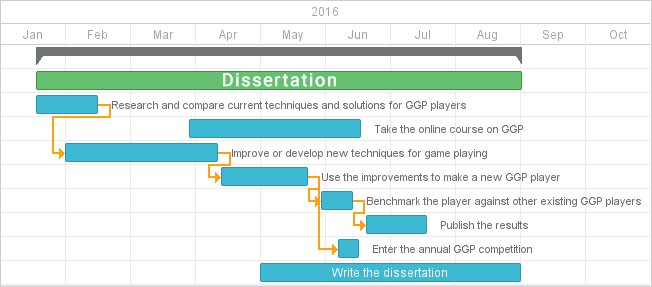
\includegraphics[scale=0.6]{images/gantt.png}
    \caption{Gantt chart for the dissertation}
    \label{fig:gantt}
\end{figure}

%%!TEX root = ../dissertation.tex

\chapter{Evaluation}
\label{chapter:evaluation}
Evaluation here...

%%!TEX root = ../dissertation.tex

\chapter{Conclusion}
\label{chapter:conclusion}
Conclusion here...




\bibliographystyle{ieeetr}
\addcontentsline{toc}{chapter}{Bibliography}

%\nocite{Mandziuk2013}
%\nocite{Swiechowski2014}
%\nocite{Swiechowski2015}
%\nocite{Mandziuk2012}
%\nocite{Finnsson2007}
%\nocite{Bjornsson}
%\nocite{Genesereth2005}
\nocite{*}

\bibliography{bibliography/dissertation}

% Glossary and Acronym List
\if\includeGlossary 1
%\printglossary[type=\glsdefaulttype]
\printglossaries
\fi

% Appendix
\appendix
%!TEX root = ../dissertation.tex

% Appendix chapters entry point
% Include the chapters below

%!TEX root = ../dissertation.tex

\chapter{GDL example: tic tac toe}
\label{appendix:gdl_example}
%[language=MATLAB,label=code:hardhist, basicstyle=\footnotesize, caption={Programa usado no laboratório}]
\lstinputlisting[language=GDL, label=gdl_example, caption={tic tac toe described in GDL}]{appendix/tictactoe.gdl}


% Back Cover
\pagenumbering{gobble}
\NewPage

\end{document}
